\chapter{Theoretische Grundlagen und verwandte Werke\label{cha:chapter2}}

\section{Patentrecht\label{sec:aaa}}

Das DPMA ist die zentrale Behörde in Deutschland, die für den Schutz von geistigem Eigentum zuständig ist und beschreibt den Nutzen von Patenten wie folgt:
\\
\\
\textit{''Mit Patenten können Sie Ihre technischen Erfindungen (innovative Produkte oder Verfahren) vor unerwünschter Nachahmung schützen. Patente belohnen ihren Inhaber oder ihre Inhaberin durch ein befristetes und räumlich begrenztes Nutzungsmonopol.''} \cite{DPMA}
\cite{Patentschutz}
\\
\\
Das deutsche Patentgesetz(PatG) \cite{PatG} regelt die rechtlichen Rahmenbedingungen für Patente in Deutschland.
Ein Patent kann gemäß §49 Abs.1 PatG von der Prüfstelle des DPMA erteilt werden. Um die Patentierbarkeit von durch künstliche Intelligenz geschaffener Computerprogramme zu prüfen fokussiert sich diese Arbeit auf die Erteilung von Patenten. Die Erteilung von Patenten lässt sich in formelle und materielle Vorrraussetzungen gliedern und aus §49 Abs.1 PatG ableiten. Das Deutsche Patent- und Markenamt prüft auf Antrag (§44 Abs.1 PatG) die formellen und materiellen Vorrausetzungen.

\subsection{Formelle Vorraussetzungen}

Zu den formellen Vorraussetzungen gehören:
\begin{enumerate}
    \item Anmeldung und Form, §§ 34, 37 und 38 PatG 
    \vspace{-0.11in} 
    \item Beseitigung gerügter Mängel, § 45 Abs. 1 PatG
\end{enumerate}

Patente müssen angemeldet werden (§ 34 Abs. 1 PatG). Gemäß § 34 Abs. 3 PatG muss die Anmeldung den Namen der/des Anmelders*in (Nr. 1), einen Antrag auf Erteilung des Patents, in dem die Erfindung kurz und genau bezeichnet ist (Nr. 2), einen oder mehrere Patentansprüche (Nr. 3), eine Beschreibung der Erfindung (Nr. 4) sowie die Zeichnungen, auf die sich die Patentansprüche oder die Beschreibung beziehen (Nr. 5), enthalten. Außerdem muss die Erfindung vollständig und deutlich offenbart sein (§ 34 Abs. 4 PatG) und nur eine einzige Erfindung enthalten (§ 34 Abs. 5 PatG). Paragraph 37 des PatG befasst sich mit der korrekten Erfinderbennenung und Paragraph 38 mit Änderungen der Anmeldung. 
\\

Sind die oben genannten formellen Anforderungen nicht erfüllt § 45 Abs. 1 PatG, wird der Anmelder aufgefordert, diese innerhalb einer bestimmten Frist zu beseitigen.

Wenn die gerügten Mängel beseitigt wurden oder es gemäß §§ 34, 37 und 38 PatG keine gerügten Mängel gibt sind die formellen Vorrausetzungen für die Erteilung eines Patents erfüllt.

\subsection{Materielle Vorrausetzungen}

Die materiellen Vorraussetungen der Patentanmeldung sind in den Paragraphen §§ 1 – 5 PatG geregelt und lassen sich unterteilen in folgende Punkte:

\begin{enumerate}
    \item Erfindung auf einem Gebiet der Technik, § 1 Abs. 1 PatG
    \begin{enumerate}
    \vspace{-0.05in}
    \item Ausschluss, §§ Art. 1 Abs. 3 PatG und § 1 Abs. 4 PatG
    \end{enumerate}
    \vspace{-0.11in} 
    \item Neuheit, § 1 Abs. 1 i.V.m. § 3 PatG
    \vspace{-0.11in} 
    \item Erfinderische Tätigkeit, § 1 Abs. 1 i.V.m. § 4 PatG
    \vspace{-0.11in} 
    \item Gewerbliche Anwendbarkeit, § 1 Abs. 1 i.V.m. § 5 PatG)
    \vspace{-0.11in} 
    \item Ausschluss, § 2 PatG)
\end{enumerate}

Eine technische Erfindung liegt laut Haedicke dann vor, wenn eine "Zugehörigkeit einer Erfindung zu einem klassischen Gebiet der Technik, d.h. insbesondere der Physik, Chemie oder Ingenieurwissenschaften
und (…) der Biologie“ besteht. \cite{(Haedicke, Patentrecht, 5. Auflage 2020, Kap. 6, Rn. 15)} Die vom Bundesgerichtshof (BGH) erstellte sog. „Rote-Taube“-Formel beschreibt technisch als  „eine Lehre zum planmäßigen Handeln unter Einsatz beherrschbarer Naturkräfte zur Erreichung eines kausal übersehbaren Erfolgs.“\cite{(Bundesgerichtshof (BGH), Urteil vom 27. März 1969, Az.: X ZB 15/67)}  Dabei genügt es „wenn die beanspruchte Lehre den Einsatz technischer Geräte umfasst“
(\cite{Bundesgerichtshof, Beschluss vom 30. Juni 2015, Az.: X ZB 1/15, III, 1. A), mit Verweis auf: BGH, Urteil vom 24.Februar 2011 -XZR121/09, GRUR 2011, 610 Rn.16)}. Aufgrund der ständigen
Fortentwicklung lässt sich der Begriff der „technischen Erfindung“ nicht abschließend definieren \cite{Haedicke, Patentrecht, 5. Auflage 2020, Kap. 6, Rn. 11).}
\\

In Paragraph 1 Abs. 3 PatG werden Gegenstände und Tätigkeiten festgelegt, die nicht als Erfindung angesehen werden dürfen. Diese sind nicht patentfähig als solche (§ 1 Abs. 4 PatG). Ausgeschlossene Erfindungen sind Entdeckungen sowie wissenschaftliche Theorien und mathematische Methoden, ästhetische Formschöpfungen, Pläne, Regeln und Verfahren für gedankliche Tätigkeiten, für Spiele oder für geschäftliche Tätigkeiten sowie Programme für Datenverarbeitungsanlagen, sowie die Wiedergabe von Informationen (§. 1 Abs. 3 PatG). 
\\

Eine Erfindung gilt als neu, wenn sie nicht zum Stand der Technik gehört. Der
Stand der Technik umfasst alle Kenntnisse, die vor dem für den Zeitrang der Anmeldung
maßgeblichen Tag durch schriftliche oder mündliche Beschreibung, durch Benutzung oder in
sonstiger Weise der Öffentlichkeit zugänglich gemacht worden sind (§ 3 Abs. 1 PatG).
Als Stand der Technik gilt auch der Inhalt nationaler Patentanmeldungen in der beim Deutschen
Patentamt ursprünglich eingereichten Fassung mit älterem Zeitrang, die erst an oder nach dem für
den Zeitrang der jüngeren Anmeldung maßgeblichen Tag der Öffentlichkeit zugänglich gemacht
worden sind (§ 3 Abs. 2 Nr. 1 PatG).Paragraph 3 Abs. 3 und 4 PatG befassen sich mit Stoffen und Stoffgemischen. Für die Anwendung von § 3 Abs. 1 und Abs. 2 PatG bleibt eine Offenbarung der Erfindung außer Betracht, wenn sie nicht früher als sechs Monate vor Einreichung der Anmeldung erfolgt ist und
unmittelbar oder mittelbar zurückgeht auf einen offensichtlichen Missbrauch zum Nachteil des
Anmelders oder seines Rechtsvorgängers (§ 3 Abs. 5 Nr. 1 PatG).
\\

Eine Erfindung gilt als auf einer erfinderischen Tätigkeit beruhend, wenn sie sich für den Fachmann
nicht in naheliegender Weise aus dem Stand der Technik ergibt (§ 4 S. 1 PatG). Gehören zum Stand
der Technik auch Unterlagen im Sinne des § 3 Abs. 2 PatG, so werden diese bei der Beurteilung der
erfinderischen Tätigkeit nicht in Betracht gezogen (§ 4 S. 2 PatG).
\\

Eine Erfindung gilt als gewerblich anwendbar, wenn ihr Gegenstand auf irgendeinem gewerblichen
Gebiet einschließlich der Landwirtschaft hergestellt oder benutzt werden kann (§ 5 PatG).
\\

Ausschluss der Patentierbarkeit besteht bei Sittenwidrigkeit (§ 2 Abs. 1 HS. 1 PatG), bei Verfahren zum Klonen menschlichen Lebewesen (§ 2 Abs. 2 S 1 Nr. 2, S. 2 PatG i.V.m. ESchG), bei Verwendung menschlichen Embryonen zu industriellen oder kommerziellen Zwecken (§ 2 Abs. 2 S 1 Nr. 3 PatG i.V.m. ESchG). In Paragraph § 2 Abs. 2 S 1 Nr. 1 PatG wird der Ausschluss in Verbindung mit Tieren behandelt.




\section{Künstliche Intelligenz\label{sec:bb}}

Der Begriff künstliche Intelligenz entstand 1956 bei einer 
Konferenz in New Hampshire. Für die Simulierung von Aspekten des 
Lernens, sowie anderer Merkmale der menschlichen Intelligenz von 
Maschinen schlägt der Wissenschaftler John McCarthy den Begriff 
„Künstliche Intelligenz“ vor. 
\cite{WasIstKuenstliche2021} \cite{WhatAIBasica}

\textit{''Künstliche Intelligenz ist die Fähigkeit einer Maschine, 
menschliche Fähigkeiten wie logisches Denken, Lernen, Planen und 
Kreativität zu imitieren''} \\ \cite{WasIstKuenstliche2020}
ist die heutige Defintion für Künstliche Intelligenz vom Europäischen Parlament 
und deckt sich fast vollständig mit der damaligen Begriffserklärung.

\subsection{KI-Typen}
KI lässt sich heutzutage in vier KI-Typen unterteilen, 
sowie in schwache und starke künstliche Intelligenz.
\\

Typ 1 KIs sind reaktive 
Maschinen welche eine einzige Aufgabe, für die sie programmiert wurden, 
erfüllen können.
\\

Typ 2 KIs können gesammelte Daten vergangener 
Situationen auf das aktuelle Geschehen anzuwenden und 
in ihren Entscheidungen berücksichtigen und sind derzeit die gängigste Form von KI.

Typ 3 KIs sind KIs mit starker künstlichen Intelligenz und 
existieren bisher nur in der Theorie. 
Sie können menschliche Emotionen wahrnehmen und ihr Verhalten daran anpassen.

Typ 4 KIs haben eine Selbstwahrnehmung und wissen selber, dass sie denken. 
\cite{stadlerKuenstlicheIntelligenz}

\subsection{Schwache und starke KI}

Schwache KIs werden für bestimmte Aufgaben eingesetzt und 
können diese meist optimal ausführen. 
Dafür sind sie jedoch auf menchliche Hilfe angewiesen, 
indem Trainingsdaten bereitgestellt und 
Parameter von Lernalgorithmen angepasst werden.

Starke KI benötigt keine menchliche Eingabe, 
sondern entwickelt sich dadurch nur schneller. 
Sie simuliert keine menschliche Intelligenz, 
sondern entwickelt eigene Intelligenz mit der Zeit. 
Dies ist besonders spannend im Hinblick auf die Frage 
des Urhebers bei Erfindungen, 
da starke KIs ohne vorherige Eingabe Erfindungen entwickeln können.
\cite{WasIstStarke2023}

Nun stellt sich jedoch die Frage,
welche KIs überhaupt 
Erfindungen erstellen können. Starke KIs sind dazu zwar in 
der Lage, aber bisher nur als theroretisches Konzept verfügbar. 
Deshalb beschränkt sich diese Arbeit zunächst auf schwache künstliche Intelligenz
mit Erfindungsfähigkeiten. Diese nennt man generative künstliche Intelligenz 
(generative KI oder generative AI).

\subsection{Generative KI}
Generative künstliche Intelligenz 
stützt sich auf Deep Learning-Modelle , 
und wird auf großen Datensätzen trainiert, um neue Inhalte zu generieren.  
Sie unterscheidet sich von diskriminativen KI-Modellen, 
die lediglich Daten sortieren und für diese Arbeit irrelevant sind. 
Die bekanntesten generativen KI-Anwendungen der letzten Jahre sind
ChatGPT und DALL-E von OpenAI, GitHub CoPilot, Bing Chat von Microsoft, 
Bard von Google, Midjourney, Stable Diffusion und Adobe Firefly. \cite{WasIstGenerative}

\subsubsection{Deep Learning, neuronale Netz und KI-Modell}

\paragraph{Deep Learning}
Um Generative KI zu verstehen hilft es Deep Learning zu verstehen.
Beim Deep Learning wird innerhalb eines neuronales Netzes in
mehreren Schichten versucht, 
das Verhalten des menschlichen Gehirns mithilfe von Dateneingaben, 
Gewichtungen und Biases zu simulieren. 
Es gibt die Eingabe und Ausgabeschicht, 
welche allgemein als sichtbare Schichten bezeichnet werden.
Eine Schicht besteht aus Neuronen, welche über Parameter 
mit der nächsten Schicht verbunden sind (Pfeile in \ref{fig:NN}).
Der Parameter Gewichtung bestimmt die Wichtigkeit des Inputs 
zum Neuron in der nächsten Schicht und der Bias die Aktivivierungssensitivität.
In der Eingabeschicht werden die Daten aufgenommen und 
in der Ausgabeschicht der entgültige Output ausgeworfen.
Die Schichten dazwischen werden als verborgene Schichten bezeichnet.
\cite{WasIstDeep2023}
\cite{KuenstlicheIntelligenz}
\\
\\
\paragraph{Neuronales Netz}
Ein neuronales Netz (Neural Network) sind die Schichten inklusive ihrer Verbindungen.
Das neuronale Netz wird trainiert indem die Eingabeschicht 
wiederholt mit Daten angereichert wird und diese immer besser klassifiziert.
Der Fortschritt entsteht dabei durch die Neugewichtung der Verbindungen 
zwischen den Schichten. 
In den Schichten werden Muster und Objekte erkannt und zu der vorherigen Schicht
wird eine Vorhersage eingegrenzt oder optimiert 
und Gewichtungen angepasst. 
Das Z in \ref{fig:NN} steht für die lineare Funktion, 
welche diese Vorhersage für die nächste Schicht berechnet.
Dieser Prozess wird als 
Vorwärtspropagierung bezeichnet. 
Entgegen dazu gibt es die Rückwärtspropagierung 
in der Fehler in den Vorhersagen ermittelt werden 
und implizit rückwärts durch die Schichten 
Gewichtungen über eine Loss Function, 
welche die Vorhersagen mit den echten Werten vergleicht, 
angepasst werden. 
Zusammen können Vorhersagen getroffen und Fehler korrigiert werden.
\begin{figure}[htb]
    \centering
    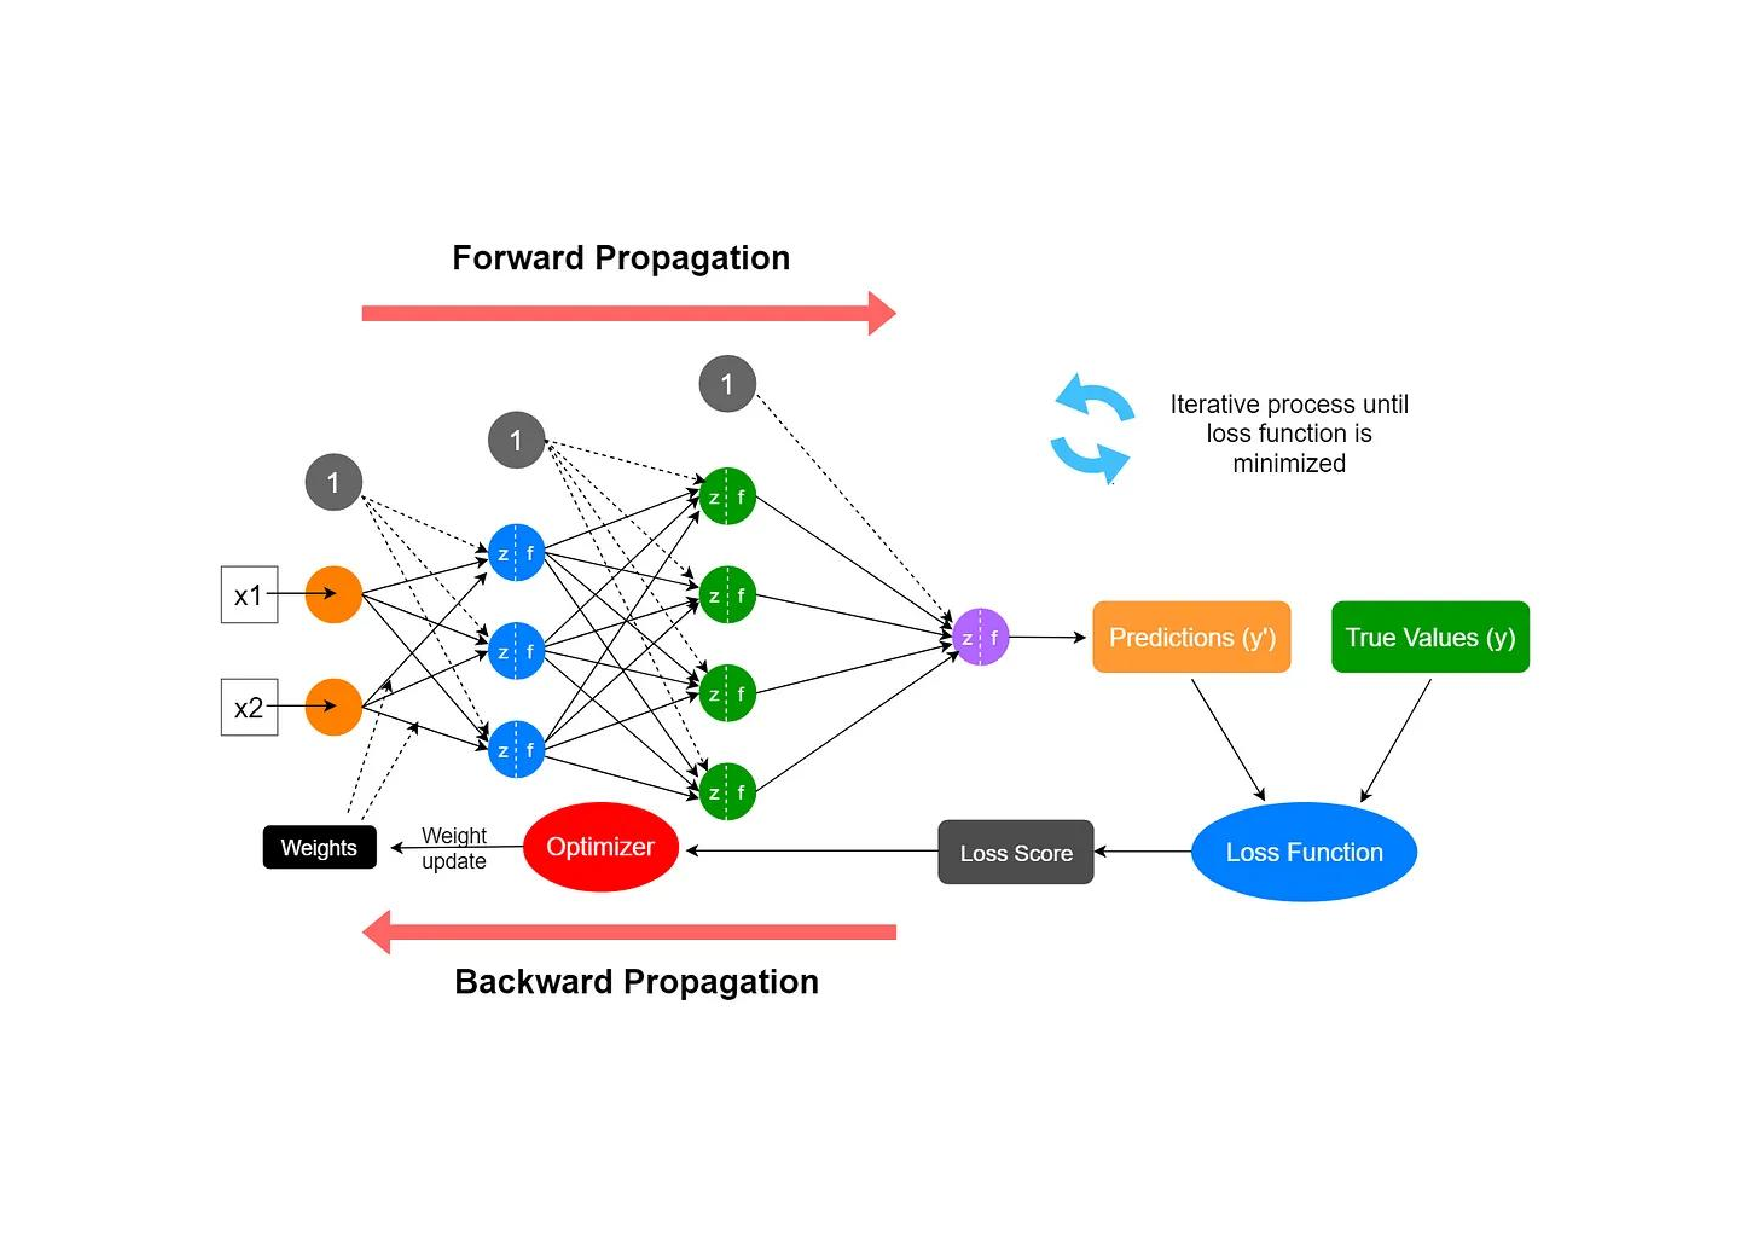
\includegraphics[width=\textwidth]{img/NeuralNetwork.pdf}\\
    \caption{ Neuronales Netz \cite{pramodithaOverviewNeuralNetwork2022a}}\label{fig:NN}
\end{figure}

  
Dabei unterscheiden sich Neural Networks in 
Faltungsneuronale Netze und Rekurrente neuronale Netze.

Faltungsneuronale Netze (CNNs), 
werden in der Erkennung von visuellen Daten eingesetzt, 
da sie Muster erkennen und so Objekte eindeutig identifizieren können.
Dabei werden neue Schichten wie die Konvolutionale Schicht, Pooling-Schicht und
die vollständig verbundene (FC(fully connected)) Schicht eingeführt. 
\cite{WasSindKonvolutionale2021}

Bei Rekurrente neuronale Netze(RNNs) werden Sequenzen in die Eingabeschicht übergeben, 
wie z.B. Sätze, 
in dem jedes Wort von dem davor und dahinter abhängig ist. 
Dies ist vorallem bei der Identifizierung von natürlicher Sprache 
und umgangssprachlichen Redewendungen nützlich und  
Standardfloskeln identifizieren und nutzen zu können.
\cite{WasSindRekurrente2023}
Heutige KI-Modelle basieren auf diesen Techniken plus einigen Verbesserungen,
wie long short-term memory (LSTM), gated recurrent units (GRUs) 
oder echo state network (ESN).
\\
\\
\paragraph{KI-Modell}
Ein KI-Modell ist das neuronale Netz mit seinen Gewichtungen. 
Vortrainierte Modelle sind z.B. GPT-3 (Generative Pre-trained Transformer Version 3).
\cite{KuenstlicheIntelligenzKI}
Durch die Eingabe eines Inputs (bei Chat-GPT zumeist Text oder Bild) 
wird ein Output in Bezug auf den Input durch das Modell erzeugt.
\\
\\
\paragraph{}
Dabei ist wichtig festzuhalten, dass bestehende KIs keine 
eigene Intelligenz besitzen, sondern diese nur Simulieren 
und auf Input angewiesen sind. Außerdem sind sie für 
verschiedene Aufgaben spezialisiert und somit als Werkzeug zu sehen. 
Die Entwicklung einer starken KI stellt eine Erschaffung von Intelligenz dar,
welche eigenständig ist und ohne Input Erfindungen erzeugt.



\newpage

\section{Computerprogramme\label{sec:comp}}

Ein Computerprogrammm ist laut ISO/IEC 2382-1:1993 
eine Kombination von Anweisungen und Deklarationen in einer
Programmiersprache, die einen Computer dazu bringen, 
Funktionen zur Lösung eines Problems auszuführen 
\cite{instituteofelectricalandelectronicsengineersinc.ISO47652010}.
Das in der Programmiersprache geschriebene Programm(Quellprogramm) wird 
mittels eines Sprachcompilers in ein in Maschinensprache geschriebenes 
Programm(Objektprogramm) aus Nullen und Einsen umgewandelt \cite{WasIstProgramm}.
Computerprogramme werden nach dem Wirtschaftslexikon Gabler in Systemprogramme
und Anwendungsprogramme unterteilt. 
Ein Anwendungsprogramm löst dabei eine bestimmte Aufgabe des Anwenders, 
wie z.B. Ticketreservierungen oder Parkraumüberwachung 
\cite{lackesDefinitionAnwendungsprogramm}. 
Während ein Systemprogramm ein Bestandteil des Betriebssystems ist und 
für den Nutzer nicht sichtbare Teile der internen Steuerung des Computer übernimmt,
wie die Orchestrierung der als nächstes zu bearbeitenden Aufgabe \cite{lackesDefinitionSystemprogramm}.
Für beide Arten von Programmen gibt es mögliche Ausprägungen, 
welche patentierbar sein können, so kann ein mögliches Szenario bei einem Anwendungsprogramm sein,
dass ein Algorithmus entwickelt wurde der in der Branche noch nicht vorhanden ist. Z.B. ein
Bildverarbeitungsprogramm, das einen neuen Algorithmus verwendet, um Bilder zu verbessern.
Oder im Falle von Systemprogrammen ein Betriebssystem mit einem 
innovativen Verfahren zur Erkennung und Verhinderung von Malware.
Welche Faktoren wichtig sind für die Patentierbarkeit von Computerprogrammen wird im nachfolgenden 
Kapitel im Abschnitt \ref{sec:patcom} dargestellt.
\paragraph{Abgrenzung zur Software}
Ein Begriff der heutzutage oft Synonym zu dem Begriff Computerprogramm benutzt wird,
ist Software. Software ist laut ISO/IEC 2382-1:1993 eine Sammlung von Computerprogrammen, 
Daten und Bibliotheken und somit ist ein Computerprogramm nur ein Bestandteil einer Software.
Software verwendet Computerprogramme als Tools um individuelle Anweisungen auszuführen 
\cite{ComputerProgrammeUnverzichtbareComputerprogramme}.
Software wird nach dem oben genannten ISO-Standard außerdem in 
Systemsoftware, Unterstützungssoftware und Anwendungssoftware unterteilt.
Systemsoftware ist Software, welche die Hardware des Computers steuert, 
wie z.B. Betriebssysteme oder Gerätetreiber. Unter Unterstützungssoftware 
fällt Software, die die Entwicklung und Ausführung von Anwendungssoftware
unterstützt, wie z.B. Compiler oder Texteditoren. Anwendungssoftware ist
Software, die für die Lösung von Problemen oder die Durchführung von Aufgaben
entwickelt wurden, wie z.B. Textverarbeitungsprogramme oder Spiele
\cite{instituteofelectricalandelectronicsengineersinc.ISO47652010}.



